% Obtained sig-alternate from http://www.acm.org/publications/proceedings-template
% This is compatible with acm_proc_article-sp
\documentclass{sig-alternate-05-2015}

\usepackage{graphicx}
\usepackage{url}
\usepackage[usenames]{color}
\usepackage{listings}
\usepackage{dirtytalk}
\usepackage[lined]{algorithm2e}


%------------------------------------------------------------------------- 
% take the % away on next line to produce the final camera-ready version 
%\pagestyle{empty}

%------------------------------------------------------------------------- 
\begin{document}

\setcopyright{acmcopyright}
\title{Limited Use Cryptographic Tokens in Securing Ephemeral Cloud Servers}

\numberofauthors{2}
\author{
% You can go ahead and credit any number of authors here,
% e.g. one 'row of three' or two rows (consisting of one row of three
% and a second row of one, two or three).
%
% The command \alignauthor (no curly braces needed) should
% precede each author name, affiliation/snail-mail address and
% e-mail address. Additionally, tag each line of
% affiliation/address with \affaddr, and tag the
% e-mail address with \email.
%
% 1st. author
\alignauthor
Gautam Kumar\\
       \affaddr{University of Washington Bothell}\\
       \affaddr{Computing and Software Systems}\\
       \email{gautamk@uw.edu}\\
% 2nd. author
\alignauthor
Brent Lagesse\\
       \affaddr{University of Washington Bothell}\\
       \affaddr{Computing and Software Systems}\\
       \email{lagesse@uw.edu}
}



\maketitle


\begin{abstract}

Many enterprises and consumers today are dependent on services which deploy their computational resources on Infrastructure as a Service (IaaS) cloud providers such as Amazon's AWS, Google's Cloud platform and Microsoft Azure. Cloud deployments at scale can have hundreds of virtual servers running and the same time sharing sensitive configuration information such as DB passwords and API Keys. This paper proposes a risk limiting architecture to safeguard against a potential information leak of sensitive configuration data using a Central Trusted Authority with hash chains as an authentication mechanism for ephemeral servers in the cloud to provide moving target defense against attackers.
\end{abstract}


\begin{CCSXML}
<ccs2012>
<concept>
<concept_id>10002978.10003022.10003028</concept_id>
<concept_desc>Security and privacy~Domain-specific security and privacy architectures</concept_desc>
<concept_significance>500</concept_significance>
</concept>
<concept>
<concept_id>10002978.10003014.10003015</concept_id>
<concept_desc>Security and privacy~Security protocols</concept_desc>
<concept_significance>300</concept_significance>
</concept>
<concept>
<concept_id>10011007.10010940.10010971.10010972</concept_id>
<concept_desc>Software and its engineering~Software architectures</concept_desc>
<concept_significance>500</concept_significance>
</concept>
</ccs2012>
\end{CCSXML}

\ccsdesc[500]{Security and privacy~Domain-specific security and privacy architectures}
\ccsdesc[300]{Security and privacy~Security protocols}
\ccsdesc[500]{Software and its engineering~Software architectures}
\printccsdesc


\section{Introduction}

Cloud infrastructure today is characterised by three difference classes of products. Infrastructure as a Service or IaaS, these are providers such as Amazon's AWS, Google's Cloud platform, Microsoft's Azure who offer on-demand compute, storage and network resource at the click of a button.  Platform as a Service or PaaS, these are providers such as Heroku and Google's AppEngine who host a developer's code and take on the responsibility of platform maintenance, i.e maintaining the compute, storage and network resource and scaling them as needed. Software as a Service or SaaS these refer to any web based application which runs on cloud infrastructure, examples include Google Apps and Microsoft's Office 365.

According to a white paper published by Microsoft \cite{harms_economics_2010}, more than 85\% work done by enterprise IT departments is towards infrastructure maintenance. IaaS providers offer enterprises a unique advantage by minimizing the effort needed to purchase and maintain physical hardware. So it stands to reason that enterprises now consider hosting their infrastructure with IaaS providers as a necessity rather than merely a competitive advantage\cite{mcafee_what_2011}.


Hosting infrastructure on the cloud comes with its own set of unique challenges and one of the primary concerns is Security. IaaS providers offer computational and storage resource on virtualized shared hardware to maximize utilization. So the essence of securing cloud systems is using multiple layers \cite{panwar_layered_2011} of security to increase an attacker's cost for taking over the system. One of the possible layer of security is using moving target defenses \cite{evans_effectiveness_2011}. 

Consider the situation where a large service provider has a number of public facing servers with access to a private, remote database.  In the case that one of those public facing servers is compromised by an adversary, the data in the private database will be vulnerable for the entire duration that the attacker has access until the attack is detected and the vulnerable server patched or removed.  The goal of our work is to drastically reduce the quantity and length of time that the attacker has to sensitive information \textit{even when we do not know that the attack has occurred}. 

In this paper we propose an implementation of moving target defense using ephemeral servers and a central trusted authority which acts on behalf an ephemeral server and proxies requests to sensitive resources such as database servers, caching servers and REST end points. Hash chains are used as an authentication mechanism by the central trusted authority. We take advantage of the limited use property of hash chains to secure authenticate ephemeral servers for a limited period of time.

% \subsection{Cryptographic hash function \cite{rogaway_cryptographic_2004}} 
% A cryptographic hash function is any one way function which meets the following requirements 
% \begin{itemize} 
% \item Preimage resistance
% \item Collision resistance
% \item Second Preimage resistance
% \end{itemize}
% 
% A hash function has preimage resistance if given a hash value $h$ it is computationally infeasible to find any message $m$ such that $h = hash(k,m)$ where $k$ is the hash key.
% 
% A hash function is collision resistant if, given two messages $m_{1}$ and $m_{2}$ it is hard to find a hash $h$ such that $h = hash(k,m_{1}) = hash(k,m_{2})$ where $k$ is the hash key.
% 
% A hash function has second pre-image resistance if given a message $m_{1}$ it is computationally infeasible to find a different message  $m_{2}$ such that $hash(k,m_{1}) = hash(k,m_{2})$ where $k$ is the hash key. The second pre-image resistance is a much harder property to achieve for hash functions. This property is closely related to the birthday problem \cite{lesser_exploring_1999}.
% 
% \begin{figure}[hbtp]
% 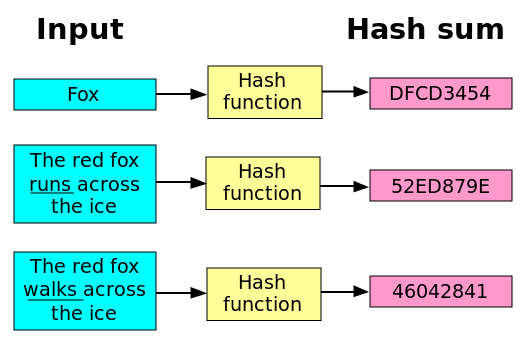
\includegraphics[scale=0.58]{hash_function.png}
% \caption{A simplified view of a hash function which represents its input and potential result. The length of the hash sum always remains the same regardless of the input size. Any small change in the input drastically changes the output.}
% \end{figure}
% 


\section{Background}


 
\subsection{Threats}

According to OWASP's Top 10 security threats, \say{Sensitive data exposure} is the $6^{th}$ most critical type of security threat in web applications as of 2013 \cite{wichers_owasp_2014}. 

Sensitive data exposure simply refers to unintended exposure of sensitive information such as passwords, social security numbers, date of birth and so on. In the context of a cloud systems sensitive information may also include credentials to access a database, email server, REST API keys and so on. These credentials are usually stored as part of a configuration file which cloud servers can use to authenticate themselves with third party services within or outside the private cloud network. 

According to a report by Risk Based Security \cite{risk_based_executives_2014} \cite{shu_privacy-preserving_2015} the number of data leaks has dramatically increased from 2012 to 2013, to the tune of \$812 million. Though sensitive data exposure in the context of cloud configurations would only constitute a small part of these leaks, leaking of such credentials can potentially lead to massive data leaks or other potential vulnerabilities being exposed to potential attackers.

Sensitive data exposure can potentially be a consequence of other threats such as cross site scripting (XSS) \cite{louw_blueprint:_2009}, Injection is the most critical threat while XSS is the $3^{rd}$ most critical threat as classified by OWASP in 2013 \cite{wichers_owasp_2014}. 

 \subsection{Cryptographic hash function } 
 A cryptographic hash function is any one way function which meets the following requirements \cite{rogaway_cryptographic_2004} 
 \begin{itemize} 
 \item Preimage resistance
 \item Collision resistance
 \item Second Preimage resistance
 \end{itemize}
 
 A hash function has preimage resistance if given a hash value $h$ it is computationally infeasible to find any message $m$ such that $h = hash(k,m)$ where $k$ is the hash key.
 
 A hash function is collision resistant if, given two messages $m_{1}$ and $m_{2}$ it is hard to find a hash $h$ such that $h = hash(k,m_{1}) = hash(k,m_{2})$ where $k$ is the hash key.
 
 A hash function has second pre-image resistance if given a message $m_{1}$ it is computationally infeasible to find a different message  $m_{2}$ such that $hash(k,m_{1}) = hash(k,m_{2})$ where $k$ is the hash key. The second pre-image resistance is a much harder property to achieve for hash functions. This property is closely related to the birthday problem \cite{lesser_exploring_1999}.
 
 \begin{figure}[hbtp]
 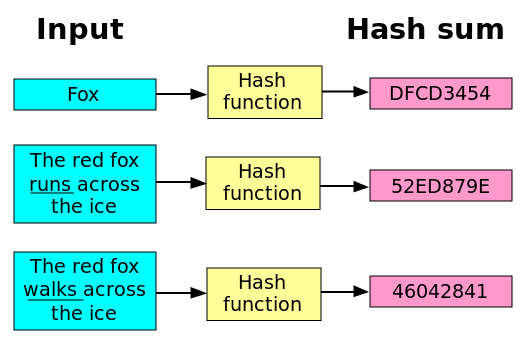
\includegraphics[scale=0.55]{hash_function.png}
 \caption{A simplified view of a hash function which represents its input and potential result. The length of the hash sum always remains the same regardless of the input size. Any small change in the input drastically changes the output.}
 \end{figure}

\subsection{Hash Chains}

Leslie Lamport \cite{lamport_password_1981} first proposed the use of hash chains in his paper on a method for secure password authentication over an insecure medium.

\say{A hash chain is a sequence of values derived via consecutive applications of a cryptographic hash function to an initial input. Due to the properties of the hash function, it is relatively easy to calculate successive values in the chain but given a particular value,it is infeasible to determine the previous value} 

A hash chain in essence is merely the successive computation of a Cryptographic hash function on a given value. 

As an example, Let $x$ be the initial password and $H$ be the cryptographic hash function.  A hash chain of length 2 would be $H^{2}(x) = H(H(x))$. A hash chain of $n$ values is denoted as $H^{n}(x)$ and the $i^{th}$ value in the chain would be computed as $x_{i} = H(x_{i-1})$.

For a given value in the chain $x_{i}$ its computationally infeasible to determine the previous value in the chain $x_{i-1}$.


\section{Proposed architecture}

The proposed architecture to defend against the threat of sensitive data exposure is to use a Central Trusted Authority (CTA) responsible for storing sensitive information. The CTA would act as a proxy and would make requests on behalf of client facing servers, refer Fig. \ref{fig:architectureoverview}.

\begin{figure}[ht]
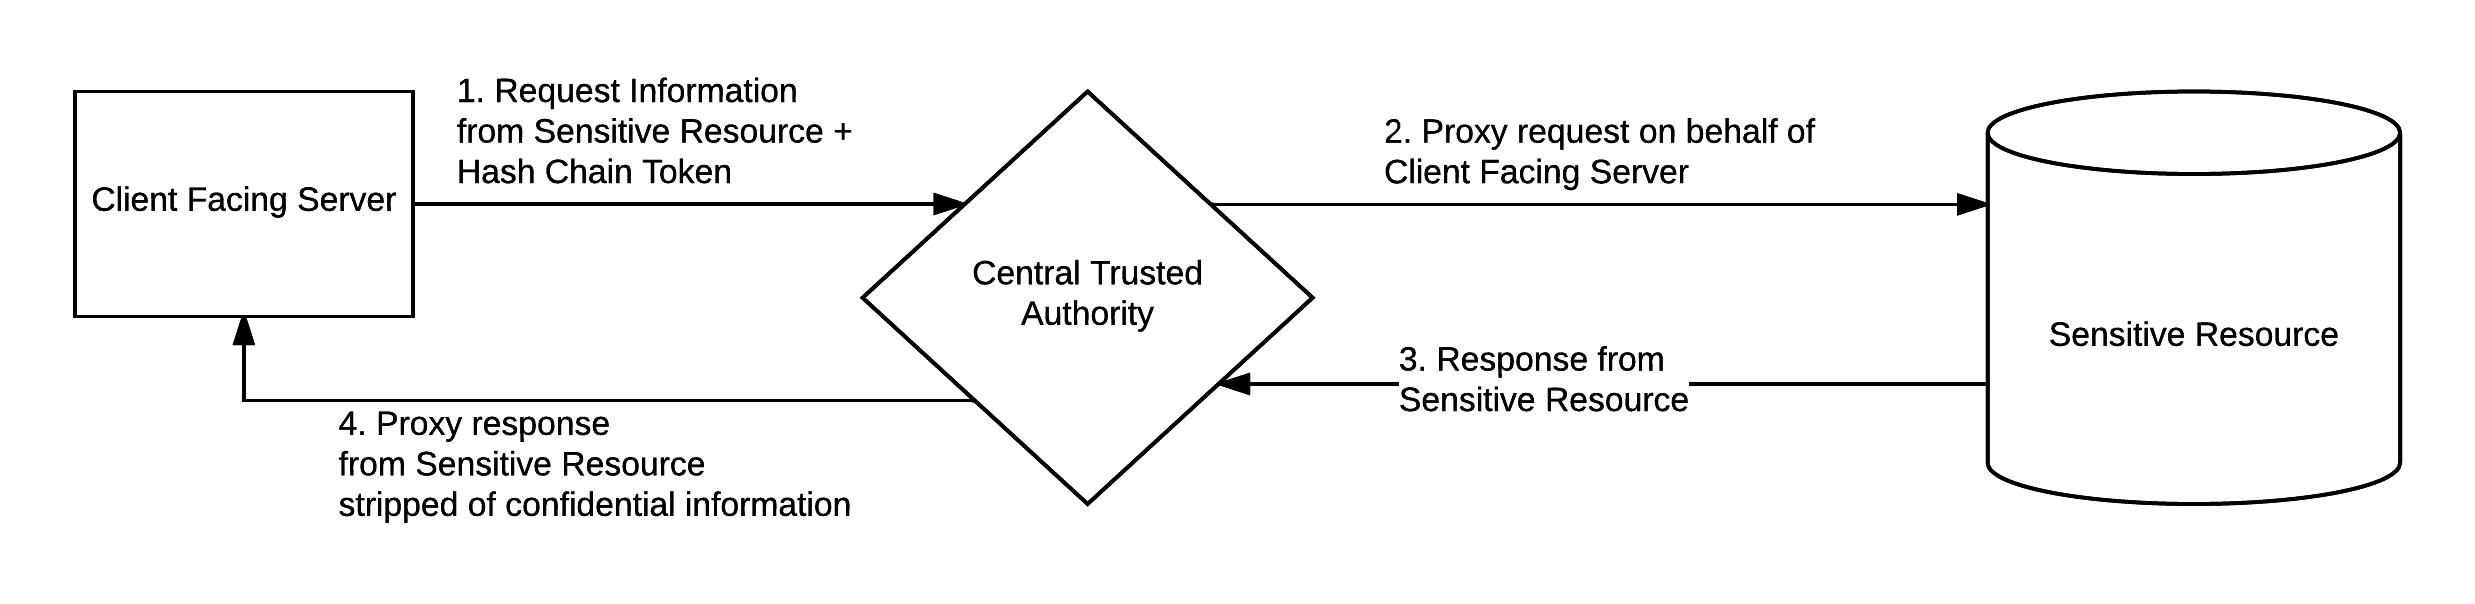
\includegraphics[keepaspectratio=true,scale=0.145]{overview_architecture.png}
\caption{Architectural overview of the system. This figure describes the three primary modules involved. The client facing server, The central trusted authority and a sensitive resource.}
\label{fig:architectureoverview} 
\end{figure}

The client facing servers would use hash chains to authenticate with the CTA. Hash chains cryptographically limit the number of times a key can be used. Limited use was intentionally selected to promote the creation of a moving target for attackers.

\subsection{Assumptions}

\begin{figure*}[!ht]
  \centering
  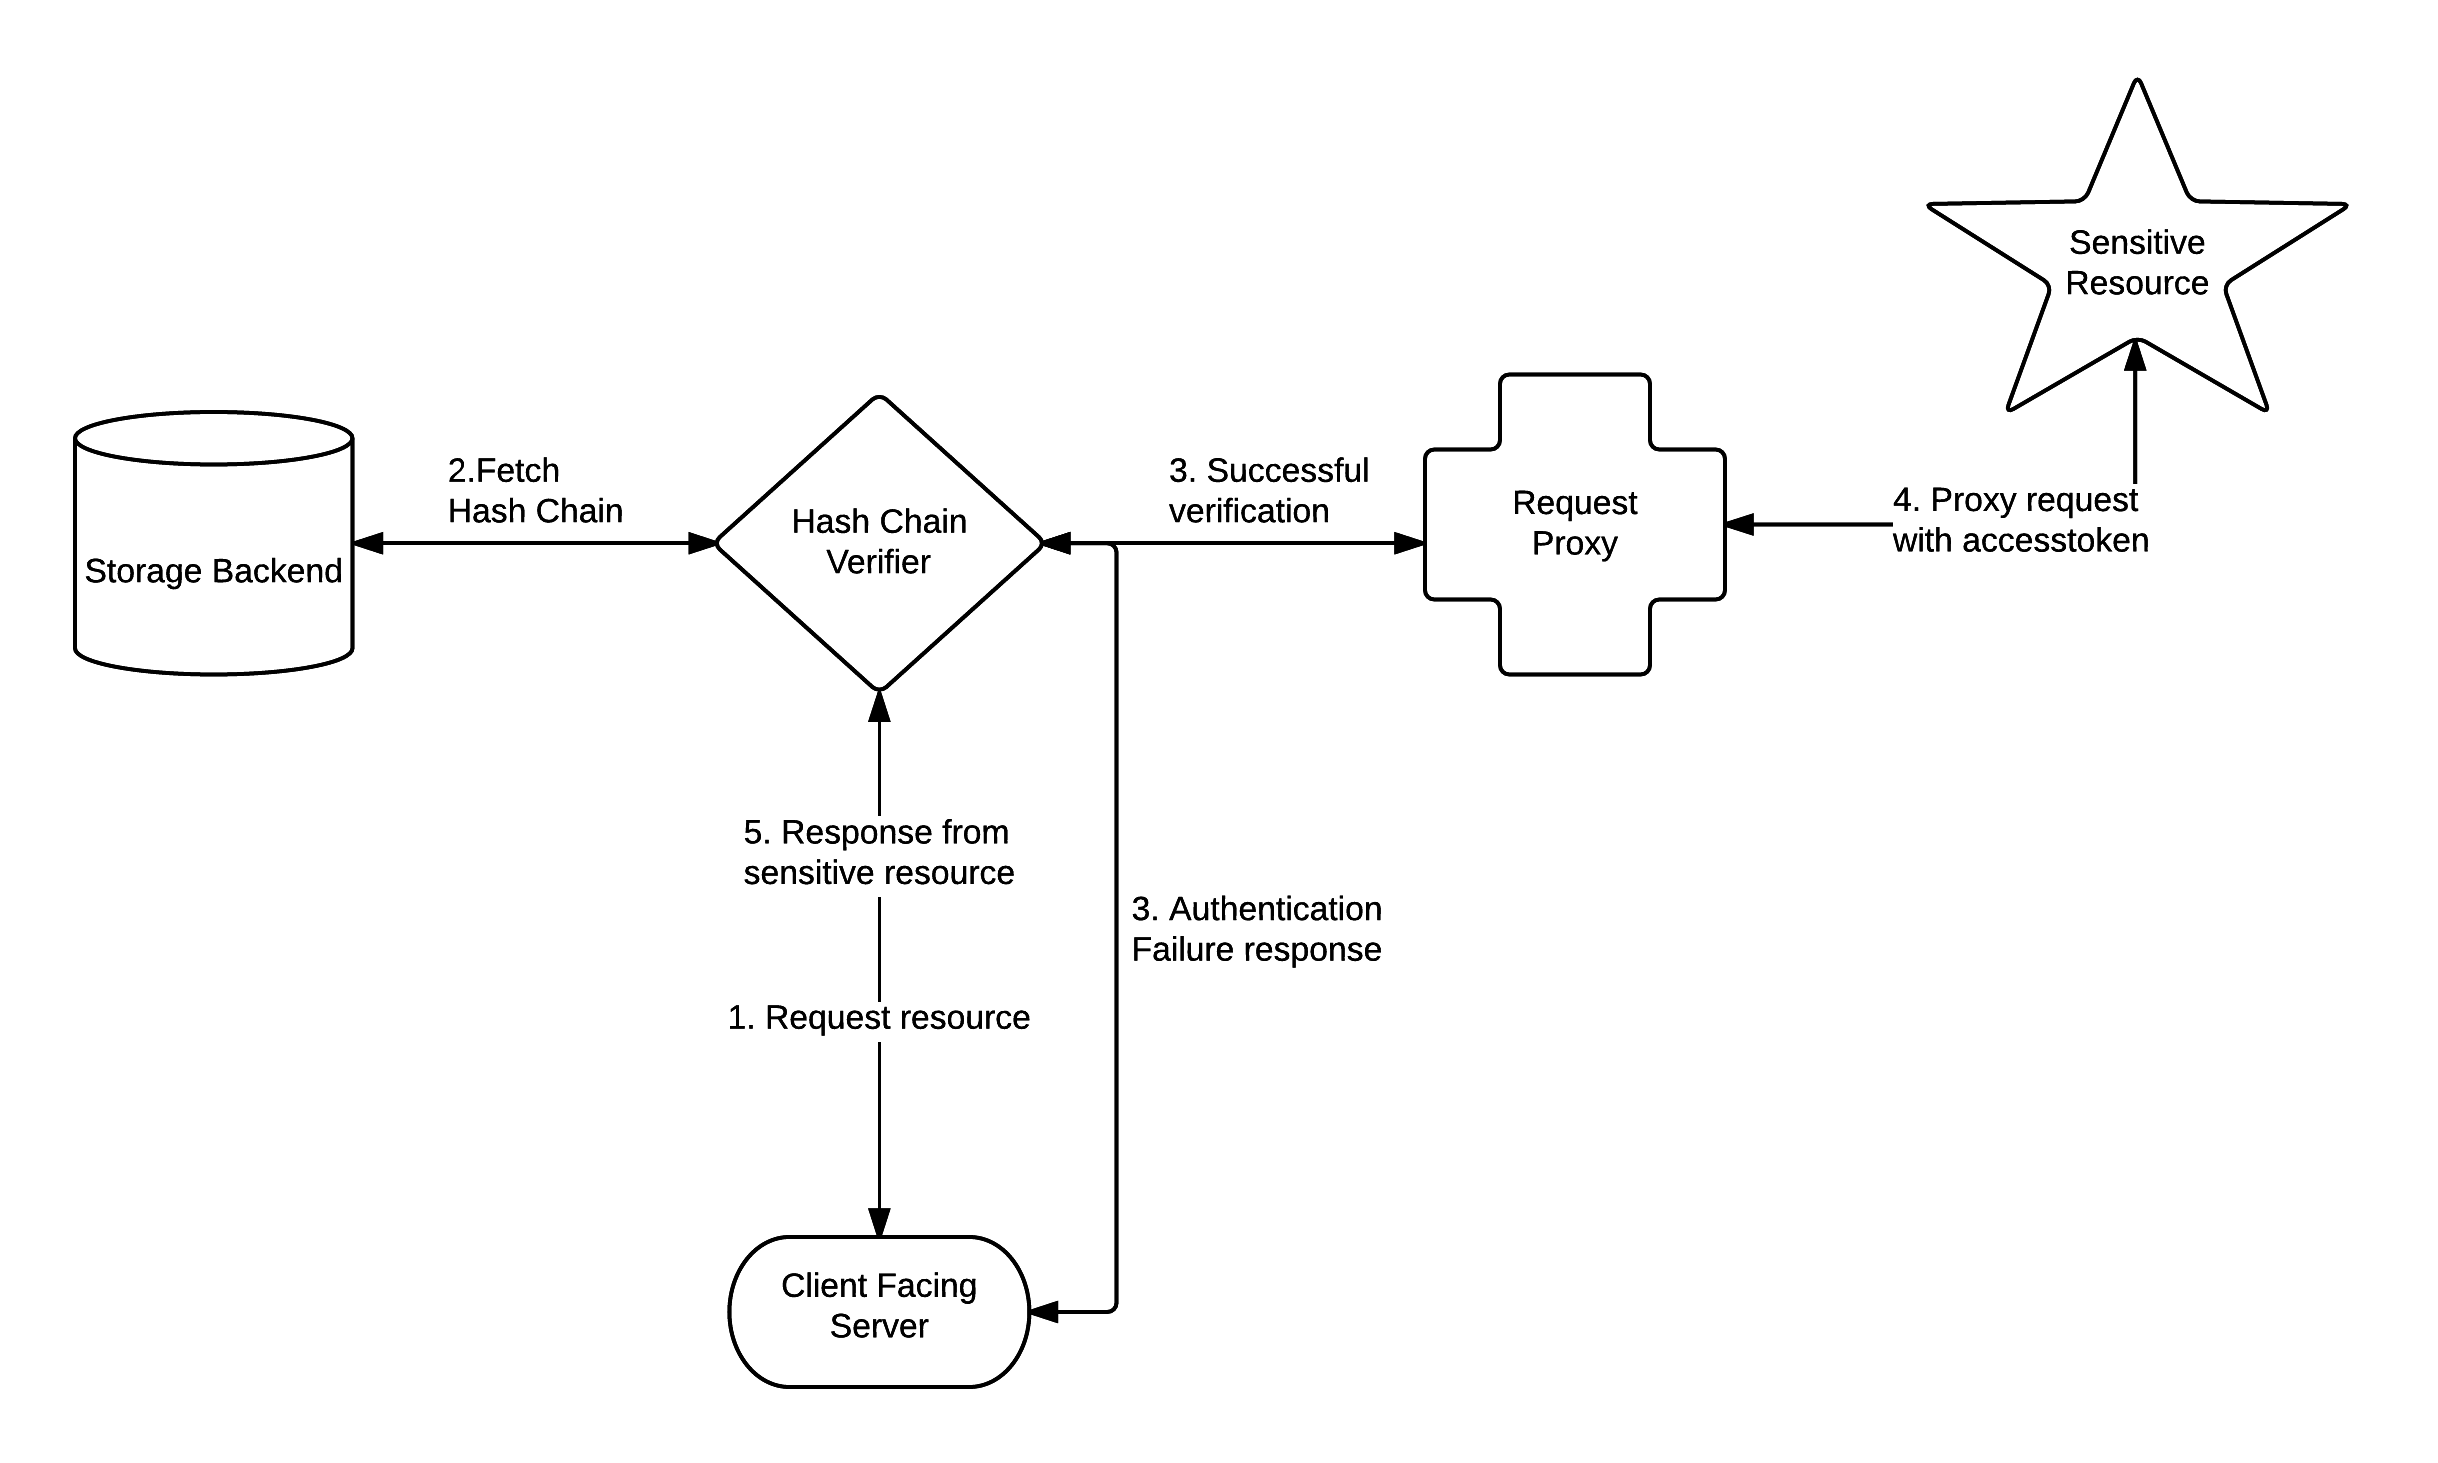
\includegraphics[keepaspectratio=true,scale=0.8]{cta_architecture}
  \caption{Architecture of the Central Trusted Authority. The CTA consists of a storage backend, a hash chain verifier and a request proxy.}
  \label{fig:ctaarchitecture}
\end{figure*}


Client facing servers are the servers which are exposed outside the private cloud network environment. These client facing servers could potentially be load balancing servers, compute servers.

The client facing servers are assumed to be ephemeral. This is common in many cloud deployments \cite{vaquero_dynamically_2011} and contributes to the moving target nature of the security architecture. Companies such as Netflix expect this behaviour with their chaos engineering architecture \cite{basiri_chaos_2016}. This allows for higher reliability of their server infrastructure.

Client facing servers are expected to shut down after their hash chain expires. This contributes to the ephemeral nature and also to moving target defense of the overall system.

\subsection{CTA Architecture and Implementation}

The Central Trusted Authority consists of three primary components, A hash chain verifier, A storage backend and a request proxy. The CTA generally performs three roles within the system which are

\begin{itemize}
\item Create new hash chain
\item Verify hash chains
\item Proxy requests
\end{itemize}

\subsubsection{Creating new hash chain}
Hash chains are created by iteratively hashing a secret key $K$, $n$ number of times. 
After the hash chain is created the CTA stores $H^{n}(K)$ in the storage backend and returns $K$ and $n$ to the client facing server. The secret key $K$ is not stored by the CTA. The client facing server can now use the the secret key $n$ number of times. This process is detailed in algorithm  \ref{algo_generating_hash_chain}.

\begin{algorithm}
\SetAlgoLined
\caption{Generating a Hash Chain}
\label{algo_generating_hash_chain}
\LinesNumbered
\KwData{Hash Chain secret $K$ and Hash chain length $N$}
\KwResult{Hash Chain $H^{N}(K)$}
$i \leftarrow 1 $\;
$H^{1}(K) \leftarrow H(K)$ \;
\While{$i <= N$}{
	$i\leftarrow i + 1$\;
	$H^{i}(K)\leftarrow H(H^{i-1}(K))$\;
}
\KwRet{$H^{i}(K)$ where $i$ equals $N$} \;
\end{algorithm}
\subsubsection{Hash chain verification}
Hash chains are used to authenticate client facing server requests which require access to a sensitive resource. The hash chain verification is detailed in algorithm \ref{algo_hash_chain_verification}.

\begin{algorithm}
\label{algo_hash_chain_verification}
\SetAlgoLined
\caption{Verification of Hash Chain authentication}
\LinesNumbered
\KwData{Authentication key $H^{i-1}(K)$ from the client}
\KwResult{Response from sensitive resource}
	Let $H_{client}^{i} = H(H^{i-1}(K))$ \;
	Let $AuthenticationData = fetch(H_{client}^{i})$ \;
	
	\eIf{AuthenticationData exists in storage backend}{
		replace $H_{client}^{i}$ with $H^{i-1}(K)$ in storage backend \;
		fetch and return response from sensitive resource \;
	}{
		return authentication failure \;
	}
\end{algorithm}


\section{Security Threats}

The proposed architecture of using a Central Trusted Authority (CTA) to proxy requests on behalf of all the clients places the CTA as a single point of failure.  We deem this an acceptable trade-off as the CTA is not a public facing system and only serves the purpose of verifying hash chains and proxying requests.  As a result, hardening its defenses against possible threats becomes an easier problem.  In our current implementation, the CTA is a single server; however, we discuss alternative designs that we are considering in section \ref{sec:future}.

Our architecture proposal does not prescribe any particular hardware / VM co-location for any components in the CTA. Thus each component can be implemented on separate machines or the CTA can be instantiated as a whole within a single VM. In this section we detail the potential security threats against each component and possible mitigation strategies.



\begin{figure*}[!ht]
  \centering
  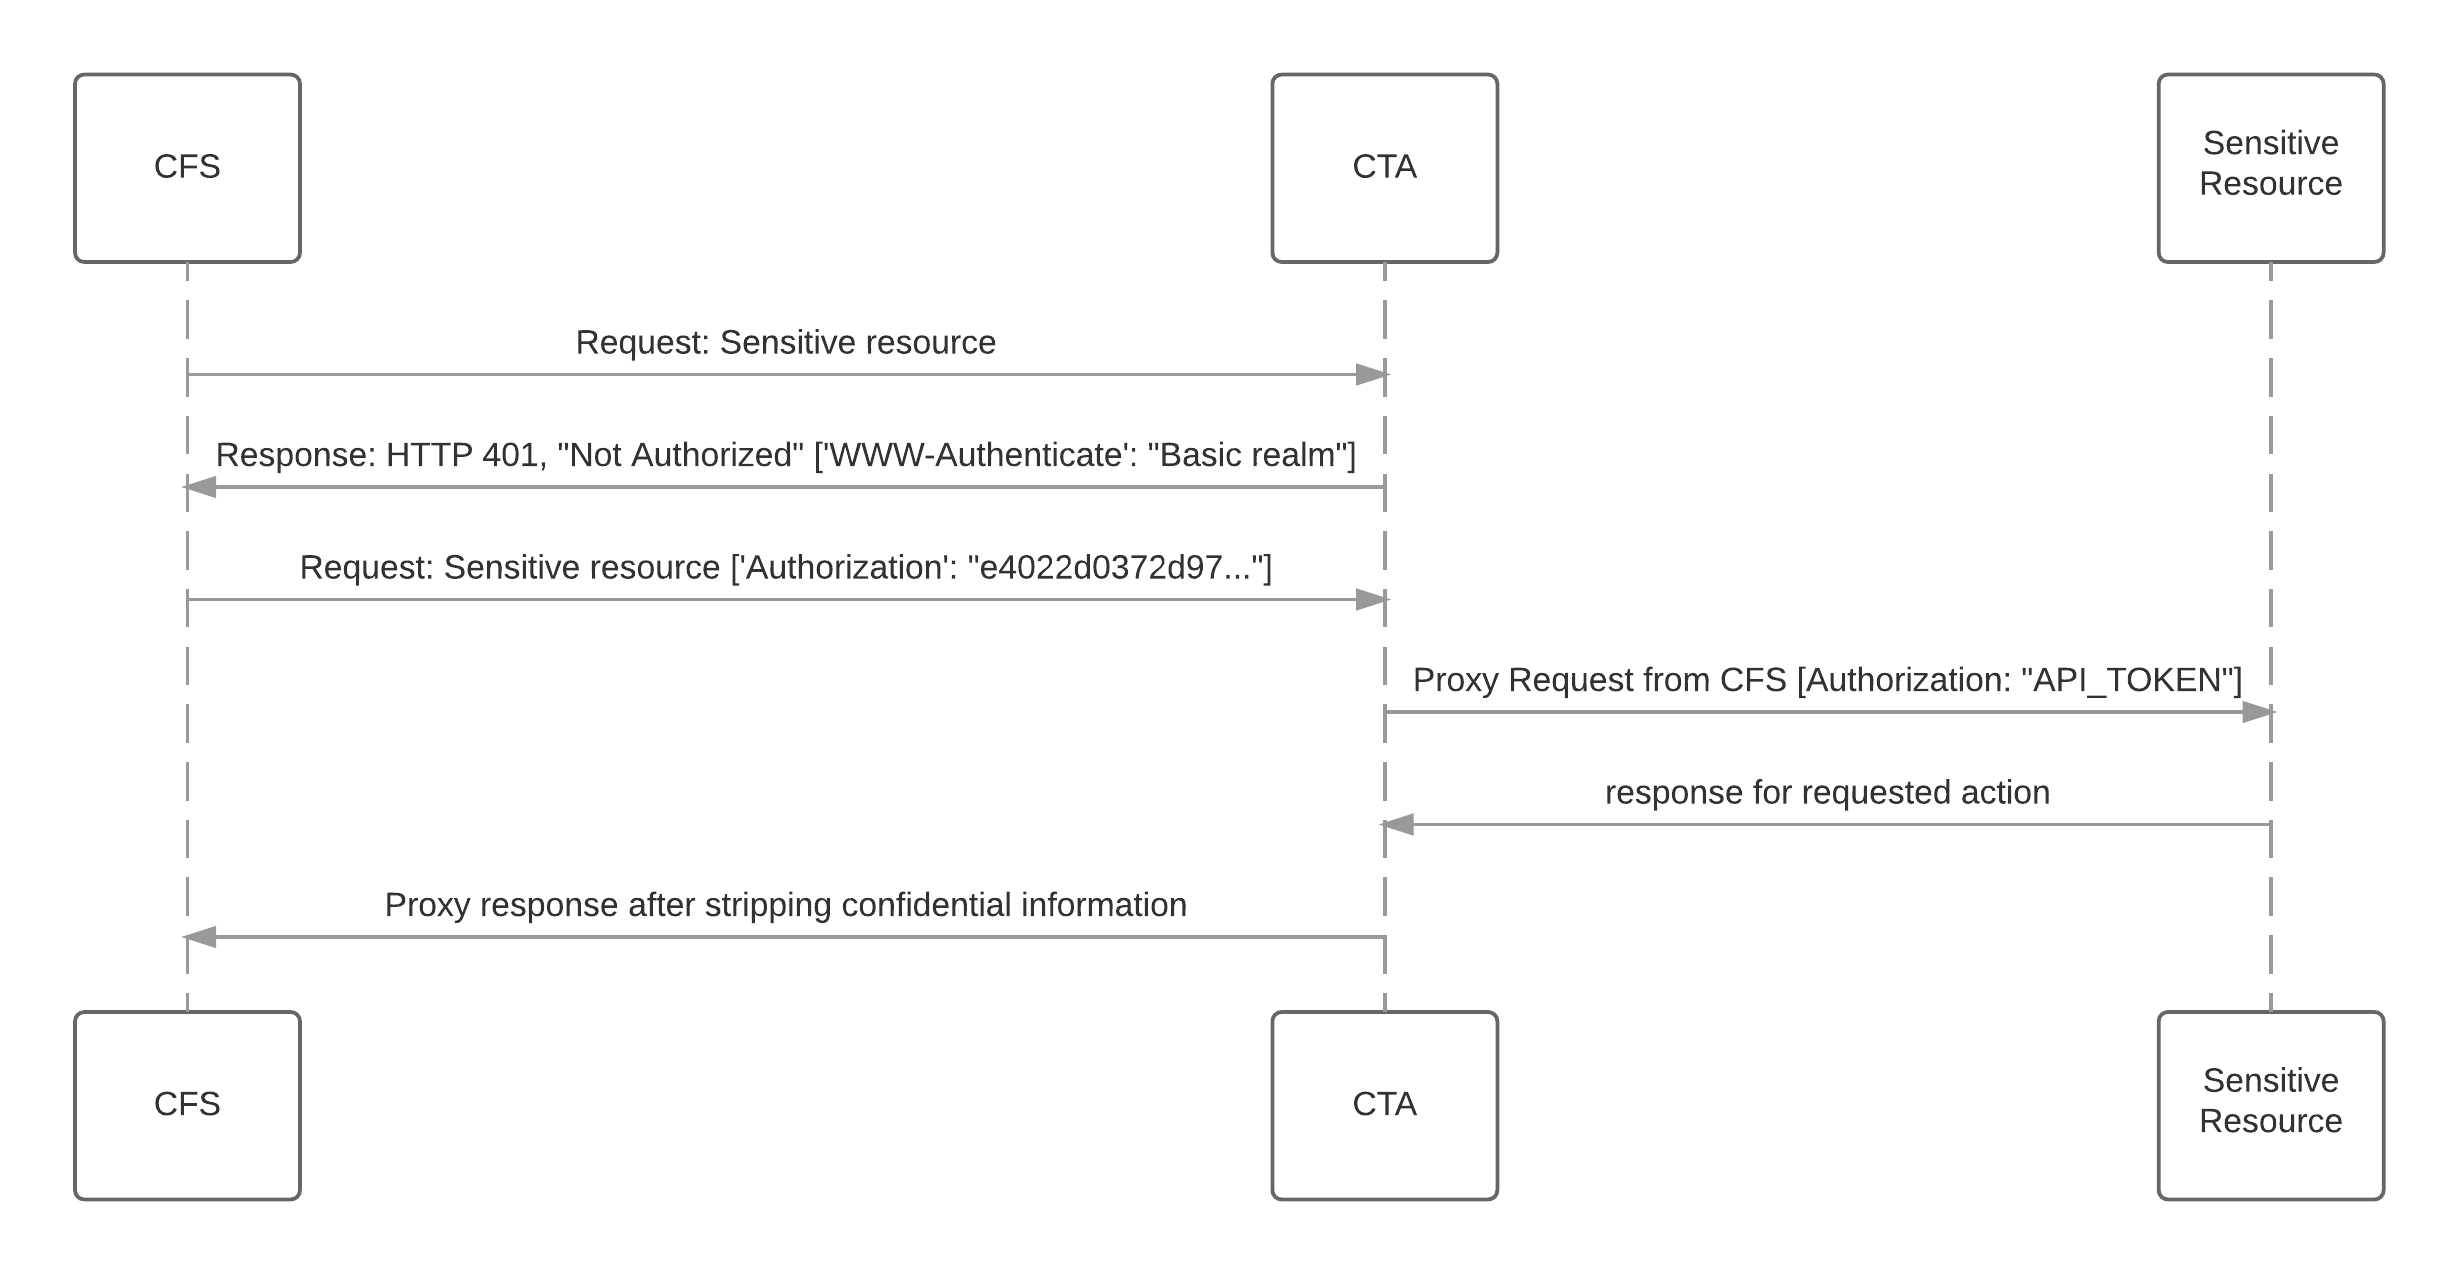
\includegraphics[keepaspectratio=true,scale=0.2]{sequence_diagram}
  \caption{Sequence diagram describing the authentication and proxying capabilities of the CTA. CFS refers to Client Facing Server while CTA refers to Central Trusted Authority}
  \label{fig:ctaarchitecture}
\end{figure*}
\subsection{Malicious Request Proxy}

The request proxy component acts on behalf of the client facing server to make a call to a sensitive resource such as an API endpoint. The request proxy is also responsible for attaching authentication information such as an API Key when contacting the API endpoint. Upon receiving a response from the sensitive resource the request proxy strips out sensitive information such as API Keys and Refresh Tokens before forwarding the response to the client facing server.Under this threat scenario the request proxy is assumed to be untrustworthy and potentially malicious.

Chen et al \cite{chen_towards_2012} propose a solution to this problem of a Malicious proxy using trusted hardware such as Trusted Platform Module (TPM) or the IBM 4758 cryptographic coprocessor \cite{parno_bootstrapping_2010}. 

Chen et al assume the proxy, the CTA in our architecture, is malicious but is incapable of modifying the underlying hardware. The CTA executable is also verified by a trusted third party to operate correctly as a proxy as described in \cite{parno_bootstrapping_2010}.

There are three primary attacks that a malicious actor may perform on the CTA. First, the attacker may try to expose the sensitive information stored, such as API keys and DB passwords, from the CTA using vulnerabilities in the CTA executable. Second, the attacker could potentially modify the requests / responses which are being proxied by the CTA. Third the attacker could potentially launch a reboot attack to inject a malicious executable after attestation to carry out one of the above attacks.

Prior work \cite{libert_tracing_2008, mccune_flicker:_2008} on preventing reboot-attacks can be leveraged to impede the attacker's ability to inject a malicious executable. The proposed architecture also allows for the CTA to be placed behind secure corporate firewalls to further limit the risk of a malicious take over by an attacker. Further work is needed to fully secure the CTA against a malicious proxy.

\subsection{Insecure Storage back-end}

Our proposed architecture can accommodate various kinds of storage backends and thus potential security threats against the storage backend may vary. 

Considering the scenario of an RDBMS system, The most common vulnerability is SQL Injection and a lot prior of work has been done to secure RDBMS systems against SQL Injection \cite{halfond_amnesia:_2005, boyd_sqlrand:_2004, halfond_classification_2006} and those techniques to drastically limit the risk of data leakage or system takeover.

Using a pre-hardened database as a service such as Amazon's RDS or Google's CloudSQL can further improve the security of our storage backend \cite{curino_relational_2011} .



\section{Performance testing}

\begin{figure}[h]
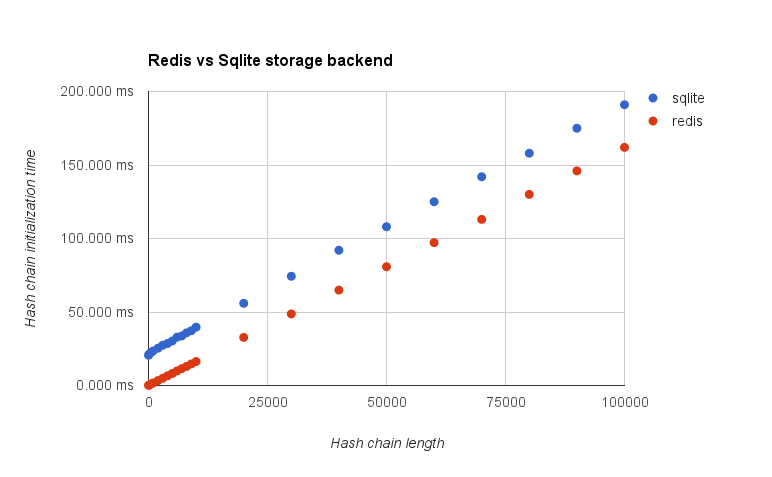
\includegraphics[scale=0.365]{performance}
\caption{Linear time complexity of the hash chain initialization. Execution platform Intel i5-5200U 2.2Ghz, 12GB RAM, SHA-512 implemented in python.}
\label{fig:performance}
\end{figure}

In our testing hash chain initialization showed a linear increase in time complexity as shown in figure \ref{fig:performance}. This is in line with our expectations for hash chain implementations. A hash chain of length 100,000 takes 150 - 200 ms to initialize based on the storage backend used. 

Using connections on Amazon EC2 US West (Oregon), we connected between machines in the same zone and connected from residential ISPs to EC2 to provide evidence that the increased workload in our proposed protocol will not drastically affect performance.  Connections within the same EC2 zone took about 0.3 ms for a round trip submission whereas the round trip time on a typical residential cable modem connection took about 25 ms to the same machine.  As a result, for small requests, we expect that the network latency will be increased by a few percent and even less, relatively, for large requests, as bandwidth within the same cloud zone can be orders of magnitude greater than most ISPs provide to both residential and commercial customers.  The only additional significant computation that occurs during runtime is the hash chain verification.  Hash chain verification is designed to be an efficient operation and the original verification process has been improved upon several times \cite{fischlin_fast_2004, yum_fast_2010}



\section{Discussion and Future work}
\label{sec:future}

\subsection{Providing moving target defense}

Green et al \cite{green_characterizing_2015} identify Unpredictability, Vastness and Revocability as some of the criteria for evaluating moving target defenses. In this section we try define how our implementation conforms to these criteria.

\paragraph*{Unpredictability} Cryptographic hash functions \cite{rogaway_cryptographic_2004} are designed to be collision resistant and comply with the avalanche effect and thus the generated sequence is highly unpredictable in nature. Hash chains can compound this effect by sequential application of the cryptographic hash function.

\paragraph*{Vastness} A secure cryptographic hash function such as SHA-256 has $128$ bit of security in its worst case scenario which translates to potentially $2^{128}$ values which can be safely computed without resistance thus offering a vast state space.

\paragraph*{Revocability} The proposed architecture allows individual chains or a group of chains to be revoked merely by purging them from the database. Further group / hierarchical revocability can be achieved using Merkle hash tree implementations as a means of Hash chain generation.

\subsection{Limitations}
The proposed architecture and implementation is designed for cloud IaaS providers such as Amazon AWS where ephemeral servers are easily managed.  As a result, the proposed system is not extensible to a cloud provider without the ability to quickly provide large number of ephemeral servers  could result is significant performance degradation.

Hash chains inherently posses certain vulnerabilities such as a Hash chain cycle and Hash chain length oracle attacks which can potentially reduce the effectiveness of the proposed architecture \cite{lee_hash_2007}. 

\subsection{Artificial diversity through DHT}

The proposed architecture lends itself well to establishing artificial diversity using a Distributed Hash Table to store the hash chains as suggested by Morell et al \cite{morrell_dht_2015}, thus further contributing to the un-predictability of the system and further limiting the risk introduced by a malicious node. 

\subsection{Future Work}
Formulating an ideal balance between server lifespan and hash chain length to optimize computational resources in a cloud system, this can be derived from current work into load balancing in cloud systems \cite{randles_comparative_2010}. Such a formulation can be used by dev ops engineers in choosing an ideal hash chain size based on the performance requirements of a cloud system.

Integrating Timed Release Cryptography \cite{chalkias_timed_2006} as a hash chain renewal mechanism to potentially increase the lifespan of a server after a certain cool off period.

A Merkle hash tree implementation middle-ware can potentially provide hierarchical authentication authorization \cite{yi_cloud_2012} capabilities to the CTA.

\section{Related work}

Confidant \cite{lyft_confidant:_2015} is a library maintained by Lyft, a transportation network company based out of San Francisco. Confidant provides an implementation of the Central trusted authority server with encryption at rest, authentication and authorization handled by AWS's Key Management Service, KMS and a storage backend of DynamoDB. This severely hampers the ability of a potential user to deploy a Confidant instance on a different cloud IaaS provider beside Amazon's AWS. 

Confidant also serves as an inspiration for the CTA component of the proposed architecture.

\section{Summary}

In this paper we propose an architecture to provide moving target defense and minimize the damage that attackers can cause by centralizing the storage of sensitive configuration information and taking advantage of the limited use property of hash chains to authenticate potentially vulnerable client facing servers. 

\bibliographystyle{abbrv}
\bibliography{css539_class_see}


%\subsection{Reliability}
%
%A lot of research \cite{dutta_smartscale:_2012} \cite{vishwanath_characterizing_2010} \cite{xuejie_reliability_2013} \cite{kumar_dynamic_2012} has been conducted into improving the reliability of cloud systems through vertical, horizontal scaling and automatic provisioning. Much of that work can be leveraged for the purpose of improving the reliability of the proposed architecture. For example, Beltr{\'a}n \cite{beltran_automatic_2015} proposes an architecture of utilizing multi-tired load balancers to improve the reliability of a service. 
%
%Large scale database deployments typically deploy databases behind a reverse proxy for load balancing and Geo distribution \cite{hoff_7_2012}. Thus a reverse proxy such as Vitess \cite{hoff_7_2012} is ideally suited to act as the CTA in such architectures.

\end{document}




